\documentclass{ximera}  
\title{Loops}  
\begin{document}  
\begin{abstract}  
We give an introduction to for and while loops.
\end{abstract}  
\maketitle

\section{Loops}

Loops are useful whenever you have an algorithm that requires multiple uses of the same step. For example, say we wanted to compute the sum $1+2+\cdots+n$ for some integer $n>0$. We have seen in a previous section that this can be done using two variables, one that tracks the current value of the sum and another that tracks whether or not our task is finished (see the flowchart below).

\begin{center}
	    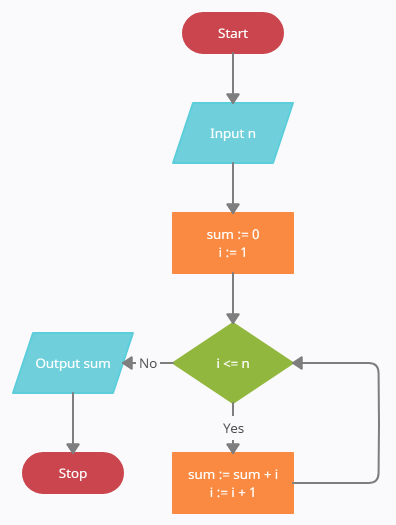
\includegraphics{gausssum.png}
\end{center}

The structure of the flowchart above is very suggestive of why we use the terminology `loop'. We will now go over two types of loops: for loops and while loops.

\section{For Loops}

The Python syntax for a for loop is as follows:

\begin{verbatim}
==============================
for variable in iterable:
        code
==============================
\end{verbatim}

In the above code, \verb|for| indicates the start of a for loop, \verb|variable| is just a variable name of your choice, \verb|in| is a keyword, and \verb|iterable| is a Python object that can be iterated over, like a list or a string. This Python code almost reads as an English statement. It is saying, for each item in \verb|iterable|, whose value we assign to \verb|variable| each time, perform the instructions given by \verb|code|.

The next few examples illustrate how \verb|variable| takes on the values of \verb|iterable|.

\begin{sageCell}
for n in [0,1,2,3]:
        print(n)
\end{sageCell}

\begin{sageCell}
for c in 'MAT1630':
        print(c)
\end{sageCell}

Below is an example of how to compute $1+2+\cdots+10$ using a for loop. 

\begin{sageCell}
n = 100
s = 0

for i in [1,2,3,4,5,6,7,8,9,10]:
        s = s + i

print(s)
\end{sageCell}

If we wanted to compute $1+2+\cdots+n$ for some large or yet unknown value of $n$, we can already see that the previous example won't cut it. We need some general way of creating useful lists of numbers. We will use the \verb|range| function to help us with this. The \verb|range| function is commonly used in for loops. The inputs for the \verb|range| function are similar to those used for list slicing. See the SageCells below for examples of how to use the \verb|range| function.

The range function with 1 argument.
\begin{sageCell}
for i in range(10):
     print(i)
\end{sageCell}

The range function with 2 arguments.
\begin{sageCell}
for j in range(2,8):
     print(j)
\end{sageCell}

The range function with 3 arguments.
\begin{sageCell}
for k in range(3,12,2):
     print(k)
\end{sageCell}

Using the \verb|range| function, we can now write a for loop that computes $1+2+\cdots+100$.

\begin{sageCell}
s = 0 
for i in range(1,101):
        s = s + i
print(s)
\end{sageCell}

We can modify, improve, and generalize the loop above. We will change out the notation \verb|s = s + i| and use \verb|s += i| instead. (The \verb|+=| operator increments whatever is on the left by whatever is on the right.) We will also create a function to compute $1+2+\cdots+n$ for any integer $n>0$.

\begin{sageCell}
def mySum(n):
        s = 0
        for i in range(1,n+1):
                s += i
        return s

print(mySum(100))
\end{sageCell}

\section{While Loops}

The Python syntax for a while loop is as follows:

\begin{verbatim}
==============================
while condition:
        code
==============================
\end{verbatim}

In the above code, \verb|while| indicates the start of a while loop, \verb|condition| is the comparison that is made to determine if the while loop is finished, and \verb|code| is executed as long as \verb|condition| holds true.

Below is an example of how to compute $1+2+\cdots+100$ using a while loop.

\begin{sageCell}
n = 100
s = 0
i = 1

while i <= n:
        s += i
	i += 1

print(s)
\end{sageCell}

Note that for a while loop, if \verb|condition| is always true, then your algorithm will never finish running. Unlike a for loop, you must be sure to update the variables associated with the condition being checked at each iteration. In the example above, omitting the line \verb|i += 1| would create an infinite loop.

\section{For or While}

A common question when learning about these two types of loops is: Which one should I use? In many cases either will work just fine. For loops are preferred when the number of times the instructions are to be repeated is known. While loops are preferred when the number of times the instructions are to be repeated is unknown.

For example, we have already seen that computing $1+2+\cdots+n$ for some integer $n>0$ can be done with a for loop using just a few lines of code. Consider the following related question: determine the smallest integer $m$ such that $1+2+\cdots+m\geq 1000$.

How large should $m$ be? In this case, a for loop may not be as helpful as a while loop since we do not know how many times to iterate. Using a while loop, we can track the value of the sum after each step. We can use the value of the sum as the condition that determines whether or not the while loop continues to iterate. 

\begin{sageCell}
s = 0
i = 1

while s < 1000:
        s += i
        i += 1
print(i-1)  # Why do we print i-1 and not i?
\end{sageCell}

\section{Problems}

Note that for the questions below, the hint contains the solution.

\begin{question}
	Write a Python function \verb|pos_floor| that computes the floor of a positive real number $x$.
\begin{hint}
\begin{sageCell}
def pos_floor(x):
        i = 0
        while i <= x:
                i = i + 1
        return i - 1
\end{sageCell}
\end{hint}
\end{question}

\begin{question}
	Write a Python function \verb|neg_floor| that computes the floor of a negative real number $x$
\begin{hint}
\begin{sageCell}
def neg_floor(x):
        i = 0
        while i > x:
                i = i - 1
        return i
\end{sageCell}
\end{hint}
\end{question}

\begin{question}
	Write a Python function \verb|my_floor| that computes the floor of any real number $x$.
\begin{hint}
\begin{sageCell}
def my_floor(x):
        if x == 0:
                flr = 0
        elif x > 0:
                flr = pos_floor(x)
        else:
                flr = neg_floor(x)
        return flr
\end{sageCell}
\end{hint}
\end{question}

\begin{question}
	Write a Python function \verb|div| that computes the number of divisors of a positive integer $n$.
\begin{hint}
\begin{sageCell}
def div(n):
        d = 0
        for i in range(1,n+1):
                if n%i == 0:
                        d = d + 1
        return d
\end{sageCell}
\end{hint}
\end{question}

\begin{question}
	Write a Python \verb|fac| function that computes $n!$ for any nonnegative integer $n$.
\begin{hint}
\begin{sageCell}
def fac(n):
        if n == 0:
                f = 1
        else:
                f = 1
                for i in range(1,n+1):
                        f = f * i
        return f
\end{sageCell}
\end{hint}
\end{question}

\section{Workspace}

\begin{sageCell}
# Use this cell to solve the above questions.
\end{sageCell}

\end{document}
